% Akulin--Karlov. Batch 02, revision v2. Source: R36 CP02 and original scans.
% Editable geometry: source semantics first; no raster is embedded in this drawing.
\documentclass[border=5pt]{standalone}
\usepackage{fontspec,unicode-math}
\setmainfont{Noto Serif}
\setsansfont{Noto Sans}
\setmathfont{STIXTwoMath-Regular.otf}
\usepackage{tikz}
\usetikzlibrary{arrows.meta,calc,intersections,decorations.markings}
\definecolor{ScienceInk}{HTML}{000000}
\definecolor{ScienceCurve}{HTML}{000000}
\tikzset{
 axis/.style={draw=ScienceInk,line width=.70pt,-{Latex[length=2.2mm,width=1.25mm]}},
 baseline/.style={draw=ScienceInk,line width=.70pt},
 trace/.style={draw=ScienceCurve,line width=1.8pt,line cap=round,line join=round},
 level/.style={draw=ScienceInk,line width=2.1pt,line cap=butt},
 virtual/.style={draw=ScienceInk,line width=1.15pt,dash pattern=on 4pt off 3pt},
 photon/.style={draw=ScienceCurve,line width=1.05pt,-{Latex[length=2.25mm,width=1.35mm]},line cap=round},
 channel/.style={draw=ScienceCurve,line width=1.05pt,-{Latex[length=2.25mm,width=1.35mm]},line cap=round},
 dim/.style={draw=ScienceInk,line width=.70pt,-{Latex[length=1.8mm,width=1.1mm]}},
 lab/.style={text=ScienceInk,font=\fontsize{15}{18}\selectfont,inner sep=2pt},
 ticklab/.style={text=ScienceInk,font=\fontsize{13}{16}\selectfont\itshape,inner sep=1pt},
 levlab/.style={text=ScienceInk,font=\fontsize{14}{17}\selectfont,inner sep=2pt},
 panel/.style={text=ScienceInk,font=\fontsize{16}{19}\selectfont\itshape,inner sep=1pt}}
\pagestyle{empty}
\begin{document}

% Source: printed p.103. E2 lies below the one-photon reference; E3 above two photons.
% Units of geometry are schematic. Both photon arrows have exactly equal lengths.
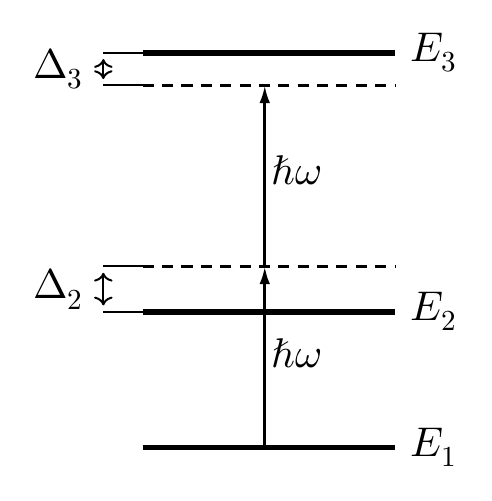
\begin{tikzpicture}[x=1cm,y=1cm]
\def\Eone{0}\def\Etwo{.75}\def\Ethree{2.18}\def\Photon{1}\def\Es{2.3}\def\Ybase{.62}
\pgfmathsetmacro\yOne{\Ybase+\Es*\Eone}
\pgfmathsetmacro\yTwo{\Ybase+\Es*\Etwo}
\pgfmathsetmacro\yThree{\Ybase+\Es*\Ethree}
\pgfmathsetmacro\yVone{\Ybase+\Es*\Photon}
\pgfmathsetmacro\yVtwo{\Ybase+2*\Es*\Photon}
\coordinate (E1) at (3.10,\yOne);\coordinate (E2) at (3.10,\yTwo);
\coordinate (E3) at (3.10,\yThree);
\coordinate (V1) at (3.10,\yVone);\coordinate (V2) at (3.10,\yVtwo);
\foreach \yy/\txt in {\yOne/{E_1},\yTwo/{E_2},\yThree/{E_3}}{
 \draw[level] (1.55,\yy)--(4.75,\yy);
 \node[lab,anchor=west] at (4.88,\yy) {$\txt$};}
\draw[virtual] (1.55,\yVone)--(4.75,\yVone);
\draw[virtual] (1.55,\yVtwo)--(4.75,\yVtwo);
\draw[photon] (E1)--node[lab,right,pos=.52] {$\hbar\omega$} (V1);
\draw[photon] (V1)--node[lab,right,pos=.53] {$\hbar\omega$} (V2);
% External compression arrows; no arrow shafts through the small gaps.
\foreach \yy in {\yTwo,\yVone,\yVtwo,\yThree}{\draw[baseline] (1.05,\yy)--(1.55,\yy);}
\draw[<->,draw=ScienceInk,line width=.72pt] (1.05,{\yTwo+.08})--(1.05,{\yVone-.08});
\node[lab,anchor=east] at (.89,{.5*(\yTwo+\yVone)}) {$\Delta_2$};
\draw[<->,draw=ScienceInk,line width=.72pt] (1.05,{\yVtwo+.08})--(1.05,{\yThree-.08});
\node[lab,anchor=east] at (.89,{.5*(\yThree+\yVtwo)}) {$\Delta_3$};
\end{tikzpicture}

\end{document}
